%************************************************
\chapter{Method validation and performance analysis on simulated data}\label{ch:simulations} 
%************************************************

\section{Simulating data with a spatial component }
Simulating data with a spatial component is a non-trivial problem. Existing methods rely on MCMC approaches as described in \cite{Chalmond89}. However, in the \platy{} in-situ data, with a relatively large number of nodes in the graph ($\sim 34,000$), this is computationally expensive \cite{belloni09}. To overcome this problem, I exploited the fact that the {\it{Platynereis}} dataset already possesses a spatial component. As outlined in Figure \ref{fig:simulationScheme}, the simulation starts by clustering the gene expression data using different values of $K$ with the HMRF method described in chapter \ref{ch:HMRF} and by storing the resulting parameter estimates. Subsequently, I use the values of the estimated parameter $\boldsymbol{\Theta}$ to simulate binarised gene expression data from $K$ clusters where, for cluster $h$, the expression of gene $m$ is simulated from a Bernoulli distribution with parameter $\theta_{m,h}$ as described in \ref{subsec:simul_non_spatial}. This non-spatial simulated data is then reintroduced in the spatial context of the biological data (\ref{subsec:simul_spatial}) leading to a simulated dataset with all parameters being fully determined. In the next paragraphs, I will describe each step of this simulation scheme.

	\begin{figure}[H]
\centerline{\includegraphics[width=0.8\linewidth]{gfx/chapter5/simulation_scheme.png}}
\caption{{\bf Simulation scheme used to generate gene expression data with a spatial component and known parameters.} The values of $\Theta$ are used to generate a dataset of clusters with the same gene expression profile as the reference. Each simulated cell is then assigned to its corresponding spatial location so that the simulated data keeps the spatial structure of the biological data.}
\label{fig:simulationScheme}
	\end{figure}
	
	\subsection{Simulating non-spatial gene expression data}\label{subsec:simul_non_spatial}
	The first step of the simulation scheme is to simulate binary gene expression data for $S=32,203$ sites and $M=86$ genes belonging to $K$ clusters. Each cluster will be assigned $N_h$ sites with $h \in [1,K]$. Given the emission model described in chapter \ref{ch:HMRF}, for each gene and each cluster, a $K \times M$ matrix $\boldsymbol{\Theta}$ is needed where each $\theta_{h,m}$ represents a Bernoulli parameter corresponding to the probability that each site in cluster $h$ expresses gene $m$.\\
	
	In order to generate a biologically coherent $\boldsymbol{\Theta}$ matrix, I applied the HMRF method to the true biological data for $K$ clusters and used the resulting $\boldsymbol{\Theta}$ matrix to simulate new data. The clustering of the biological data also generates the number of cells per cluster $N_h, \forall h \in K$.\\
	
	Once the parameters values are available it is relatively straight forward to simulate a vector of gene expression for the $N_h$ sites in each cluster.
	\subsection{Introducing a known spatial context}\label{subsec:simul_spatial}
	Each simulated data point is then assigned to the same spatial location as the corresponding ``cube" in the biological dataset, meaning that both the simulated and the biological datasets have the same neighbouring graph. By using simulated gene expression data equivalent in the same spatial context as the true data, the hypothesis is that the set of parameters $\boldsymbol{\beta}$ will stay relatively stable when the simulated data is clustered. Consequently, the values of $\boldsymbol{\beta}$ obtained after clustering the true data may be used as reference values.
	\subsection{Expected results}\label{subsec:expected_simul_results}
	Given this simulation scheme, the expected result after clustering the simulated data, is a strong conservation between the ``true" values $\hat{\boldsymbol{\psi}}$ obtained from clustering the biological data and the estimated values $\widetilde{\boldsymbol{\psi}}$ obtained after clustering the simulated data.\\

\section{Comparing clustering results using the Jaccard similarity coefficient}
	\subsection{Theoretical problem in comparing clustering results}
To compare clustering results, several metrics exist to estimate the similarity between two lists of clusters. One of the most widely used ones is the Jaccard coefficient \cite{jaccard1901}. For two clustering results, for instance the output of two approaches when clustering the same data $A$ and $B$, the Jaccard coefficient quantifies the similarity between $A$ and $B$. In other words, the higher the Jaccard coefficient between $A$ and $B$, the more similar the two clustering sets are. $J(A,B)$ is defined as: 
\begin{align*}
J(A,B) = \frac{|A \cap B|}{|A \cup B|}
\end{align*}
Although theoretically very simple, in practice computing this metric is not trivial. Indeed, depending on the clustering method used and on the initialization, even if the clustering results are 100\% identical, they may be misaligned.\\

This means that for method $A$ \emph{cluster~1} could for example be \emph{cluster~5} in method $B$. In order to compute the Jaccard coefficient and compare clustering results, it is necessary to be able to align different sets. This problem may be solved by computing the Jaccard coefficient for all possible combinations of clusters between $A$ and $B$. However, computationally when $K$ increases, computing the Jaccard coefficient for this exponentially increasing number of combinations quickly becomes expensive. Consequently, I developed a similarity specificity matrix approach as described in the next paragraph to align the clustering results before computing the Jaccard coefficient.


	\subsection{Alignment via similarity-specificity matric}
The ``count" matrix $D$ and the ``similarity/specificity" matrix $H$ for comparing two clustering outputs, $z$ and $z'$, each with $K$ clusters, so that $z = \bigcup_{h \in [1,K]} c_h $ and $z' = \bigcup_{h \in [1,K]} c'_h$ are defined as:
\begin{align*}
D &= \left( \begin{array} {ccc}
|c_1 = c'_1| & \ldots  & |c_1 = c'_K|\\
\vdots & \ddots & \vdots\\
|c_K = c'_1| & \ldots & |c_K = c'_K| \end{array} \right)\\
\text{and}\\
H_{ij} &= \frac{D_{ij}}{\sum_{a} D_{aj} \sum_{b} D_{ib}} 
\end{align*}
With $z$ the set of reference clusters (in the case of the simulation study, $z$ is the set of ``true" clusters obtained after clustering the biological data), for each row of the matrix $H$, the column with the highest value is selected as the corresponding cluster.\\

In the case of two sets of clusters being extremely similar the alignment is successful and no information is lost. However some errors may arise if the two cluster sets are quite different. For example if one cluster $h_{z_1}$ in $z$ is split into two clusters $h_{z'_4},h_{z'_5}$ in $z'$, the alignment process will assign them both to $h_{z_1}$, meaning that, because $K$ is the same for $z$ and $z'$ one cluster in $z$ will have no corresponding clusters in $z'$. In such cases, some information will be lost during the alignment process.\\

This sort of error is very hard to avoid without controlling the initialization of the clustering, which would bias the results. Therefore, the Jaccard coefficient will not necessarily be linearly correlated with the similarity between the reference clusters and the clusters under study, instead it will have a tendency to worsen faster than the dissimilarity due to the alignment step. It remains however a good indicator of the divergence between clustering sets. An example of cluster alignment is shown through the values of $\boldsymbol{\Theta}$ by comparing  figures \ref{fig:theta_valid_non_aligned} and \ref{fig:theta_valid_aligned}.\\

Now that I have established a method to compare cluster sets, I need to validate the correct estimation of the model's parameters, as described in the next section.


\section{Validation of parameters estimation and model selection}
	\subsection{Estimation of $\boldsymbol{\Theta}$}
	To validate the consistency in estimating the values of $\boldsymbol{\Theta}$, I compare the ``true" values used to simulate the data with the values obtained after clustering the simulated data.\\
	
	A simple example with $K=6$ is presented in Figure \ref{fig:theta_valid}: each cell of the heatmaps $HM_{h,h'}$ with $h,h' \in K$ represents the mean of the vector of pairwise differences $\theta_{h,m} - \theta_{h',m}$. Figure \ref{fig:theta_valid_non_aligned} shows these values before alignment and Figure \ref{fig:theta_valid_aligned} after. As expected, after alignment the small values are aligned in the diagonal showing that each cluster $h'$ exhibits highly similar values of $\boldsymbol{\Theta}$ compared to its corresponding cluster $h$ in the reference.\\
	 
\begin{figure}[bth]
        \myfloatalign
        \subfloat[``Proximity" between values of $\boldsymbol{\Theta}$ before alignment]
        {\label{fig:theta_valid_non_aligned}
        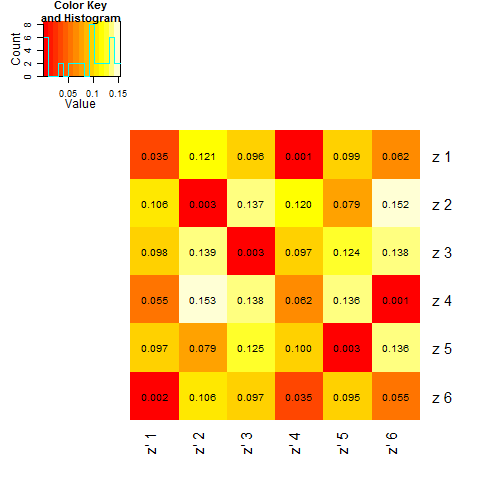
\includegraphics[width=.45\linewidth]{gfx/chapter5/heatmap6.png}} \quad
        \subfloat[``Proximity" between values of $\boldsymbol{\Theta}$ after alignment]
        {\label{fig:theta_valid_aligned}%
         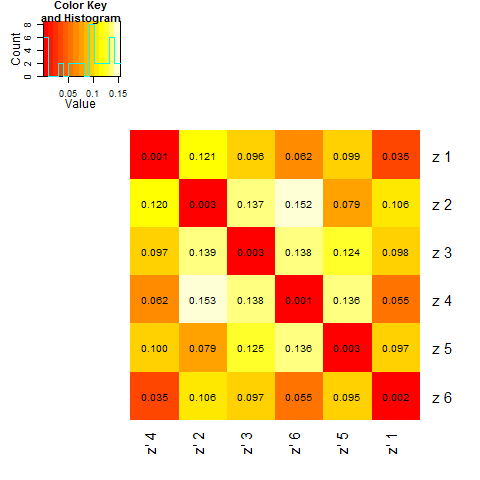
\includegraphics[width=.45\linewidth]{gfx/chapter5/heatmap6_aligned.png}}
        \caption{Validating the estimation of $\boldsymbol{\Theta}$ for $K=6$. On the x axis are shown the 6 clusters obtained after clustering the simulated data. On the y axis are shown the 6 ``true" reference clusters. Each cell of the heatmap corresponds to the mean of the absolute pairwise (with respect to the 86 genes considered) difference between ``true" and simulated $\boldsymbol{\Theta}$ values. A small number means that the difference between the reference $\boldsymbol{\Theta}$ values and the ones obtained after clustering the simulated data is very small.}\label{fig:theta_valid}
\end{figure}
	
	It is also interesting to note that comparing the similarity between the inferred and true clusters with the Jaccard coefficient implicitly assesses the accuracy of the estimation of $\boldsymbol{\Theta}$: if the inferred and true clusters are identical, the estimates of $\boldsymbol{\Theta}$ must be equal to the true values. In practice, a Jaccard coefficient of 1 implies perfect agreement. Figure \ref{fig:methodComparison} shows the value of the Jaccard coefficient for several clustering methods including the HMRF (red points). The very high value of the Jaccard coefficient suggests that the values of $\boldsymbol{\Theta}$ are consistently estimated for $K \in [4,80]$ (see \ref{sec:method_comparison} for the full description of figure \ref{fig:methodComparison})\\
	

	\subsection{Estimation of $\beta$}\label{subsec:beta_estimation}
	To determine how accurately the values of $\boldsymbol{\beta}$ are estimated, I compare the true and inferred mean values of $\boldsymbol{\beta}$ for different values of $K$, as shown in Figure \ref{fig:beta_validation} (red and green dots). I chose to compare the mean values instead of comparing $\boldsymbol{\beta}$ in a pairwise manner because of the alignment errors descibed in the previous paragraph. Indeed, for example if one true cluster is split in two after clustering the simulated data, there isn't a simple rule about how the value of $\beta$ should be distributed between the two resulting cluster. In this context using the mean value allows a consistent comparison of the overall value of $\boldsymbol{\beta}$, even though the sensibility for extreme values is lost.\\

	 Analysing Figure \ref{fig:beta_validation}, I observe that the values of $\boldsymbol{\beta}$ increase with $K$, which is to be expected since more clusters implies the existence of more transition areas, thus making an increase of $\boldsymbol{\beta}$ necessary to maintain the optimal spatial coherency of the model.\\
	
	Interestingly, Figure \ref{fig:beta_validation} also shows a slight but consistent underestimation of $\boldsymbol{\beta}$. This can be explained by noting that the simulation scheme used may reduce the spatial coherency within clusters. Specifically, as illustrated in Figure \ref{fig:beta_error}, clusters may not display homogeneous expression of a given gene: instead, depending upon the value of $\theta$, a gene will be expressed only in a fraction of cells. In reality, the cells in which such genes are expressed may have a coherent spatial structure within the biological cluster that is lost in the simulation, thus explaining the consistently smaller value for $\boldsymbol{\beta}$ that are estimated.\\
	
	 To explore this further, I performed a second simulation using the parameter values estimated from the first simulation as a reference. In this context no further loss of spatial coherency was expected, which was indeed confirmed as shown by the blue curve in Figure \ref{fig:beta_validation}.\\
	
	\begin{figure}[H]
\centerline{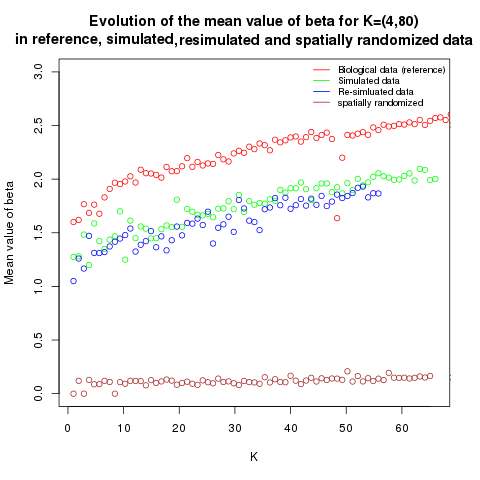
\includegraphics[width=0.8\linewidth]{gfx/chapter5/beta_valid.png}}
\caption{{\bf Validating the estimation of beta.} This figure shows the evolution for $K \in [4,80]$ of the mean value of $\beta$ across all the clusters. The red dots represent the biological data clustering (i.e the reference in our simulations scheme). The green dots represent the results obtained after clustering simulated data, which shows an underestimation of $\beta$. To confirm that this underestimation come from the simulation scheme and not the clustering method, the simulated data was used as the reference to generate a ``second generation" of simulated data, suppressing the simulation scheme bias (see Figure \ref{fig:beta_error}). The results of this re-simulation are shown by the blue dots, which exhibit no underestimation of $\beta$. Finally the brown dots represent the mean value of $\beta$ on the same simulated data but spatially randomized, as expected the $\beta$ are now estimated to $0$.}
\label{fig:beta_validation}
	\end{figure}
	
	\begin{figure}[H]
\centerline{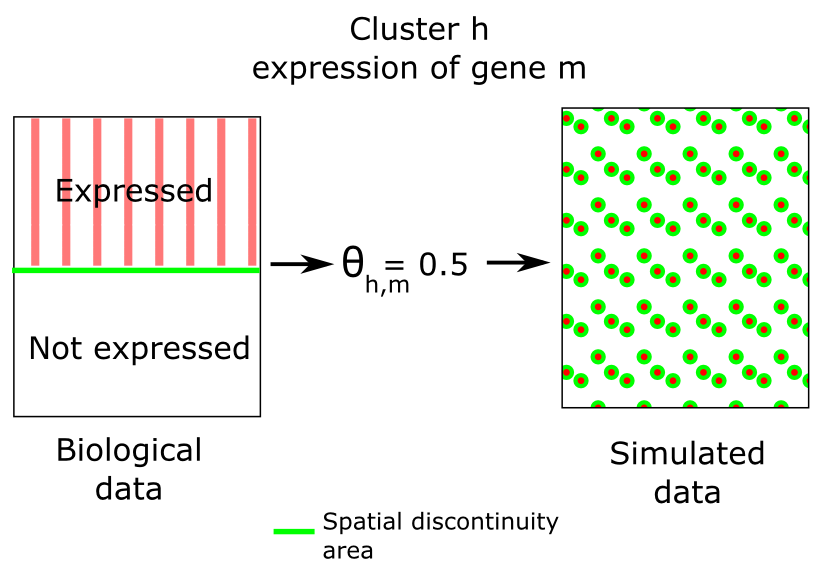
\includegraphics[width=0.8\linewidth]{gfx/chapter5/beta_error.png}}
\caption{{\bf Decrease in spatial coherency due to the simulation scheme.} For an example cluster $h$, gene $m$ may only be expressed in half of the cells. This will yield $\theta_{h,m} = 0.5$. However, in the biological data, the cells expressing gene $m$ may be spatially coherent (i.e., located close to one another), leading to a reduced area of expression discontinuity (the green line). By contrast, in the simulated data the expression of such a gene will lose its spatial coherency, leading to an increased area of expression discontinuity. The number of cells having a neighbour with some differences in the gene expression pattern is directly linked to the value of $\beta_h$ through the energy function described in chapter \ref{ch:HMRF}. This explains the underestimation of $\boldsymbol{\beta}$ observed in Figure \ref{fig:beta_validation}.}
\label{fig:beta_error}
	\end{figure}

To validate further our estimation of $\boldsymbol{\beta}$, I randomized the coordinates of the simulated ``cubes" to lose any spatial component before re-clustering the data. As expected, we observed that the estimates of $\boldsymbol{\beta}$ were very close to $0$ for all clusters (Figure \ref{fig:beta_validation}, brown dots) , as well as there being very similar Jaccard coefficient values (relative to the true values) for the independent mixture and the MRF model as shown in figure \ref{fig:methodComparison}B. Both of these observations provide confidence in our assertion that the model is able to consistently estimate the values of $\boldsymbol{\beta}$ and that the spatial component of the model plays an important role in the fit.\\
	
	\subsection{Choosing K}
	
Finally, assessing the ability of the model to choose the correct number of clusters, $K$ is crucial. To this end, the ``true" number of clusters underlying the simulated data $\hat{K}$ was compared to the inferred value, $\widetilde{K}$ obtained after applying the BIC method (see chapter \ref{ch:HMRF}). The results for two representative choices of $K$ are shown in Figure \ref{fig:simulatedK} and demonstrate that our clustering approach, in conjunction with the BIC, is able to accurately determine the optimal number of clusters.\\

	\begin{figure}[H]
\centerline{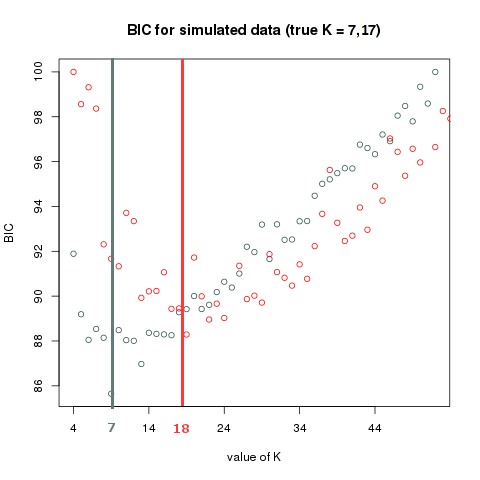
\includegraphics[width=0.8\linewidth]{gfx/chapter5/simulated_k.png}}
\caption{{\bf Estimating the BIC from the simulated data.} The BIC is plotted on the y-axis for different values of K on the x-axis. The red and the grey points correspond to the BIC estimated when the underlying data have 17 and 7 clusters, respectively. The minimum BIC value is 18 and 7, respectively, suggesting that the MRF approach in conjunction with the BIC well estimates the optimal number of clusters.}
\label{fig:simulatedK}
	\end{figure}

\section{Method performance and initialization}\label{sec:method_comparison}
As pointed out previously, initialization is a key step of the HMRF clustering. Working on the simulated data allows a comparison of clustering results generated with a variety of initialization schemes.
	\subsection{The EM principle and local maximum}
As explained in chapter \ref{ch:HMRF}, the HMRF clustering I developed relies on a Maximum Posterior Marginal (MPM) approach, and the EM algorithm is used to estimate the unknown parameter values. The likelihood function that needs to be maximised may possess many stationary points of different natures. Thus, convergence to the global maximum with the EM algorithm, depends strongly on the parameters initialisation. To overcome this problem, different initialisation strategies have been proposed and investigated (see for instance \cite{biernacki03,karlis03,mclachlan04}).\\

Indeed, if the procedure is initialized with a set of clusters that are close to a local maximum in the likelihood function, the EM algorithm will converge to this local maximum and will never reach the global maximum of the model.

	\subsection{Random initialization vs Hclust initialization}
	To shed some light on the initialization scheme issue I compared two theoretically opposed initialization schemes :
\begin{itemize}
	\item A random approach: 10.000 random initialization were generated for $K \in [4,70]$ and for each, the initial likelihood of the model was computed. The initialization with the highest initial likelihood was selected to start the EM algorithm.
	\item A directed approach: the data were clustered using the non-spatial hClust method described in chapter \ref{ch:non_spatial_clustering_visualization} and the resulting set of clusters were used to initialize the EM algorithm.
\end{itemize}

The results are shown in figure \ref{fig:methodComparison} (black and green dots on panel A). Looking at the effect of the initialization scheme on the quality of the resulting clusters via the Jaccard coefficient for $K \in [4,70]$ it is clear that, unsurprisingly, considering that the EM algorithm does not guarantee to reach the global maximum, the random initialization scheme performs better than the directed initialization scheme. Indeed, for the HMRF randomly initialized, the average Jaccard coefficient is around $0.8$ when it averages only $0.6$ when initialized with hClust.\\

	\begin{figure}[h]
\centerline{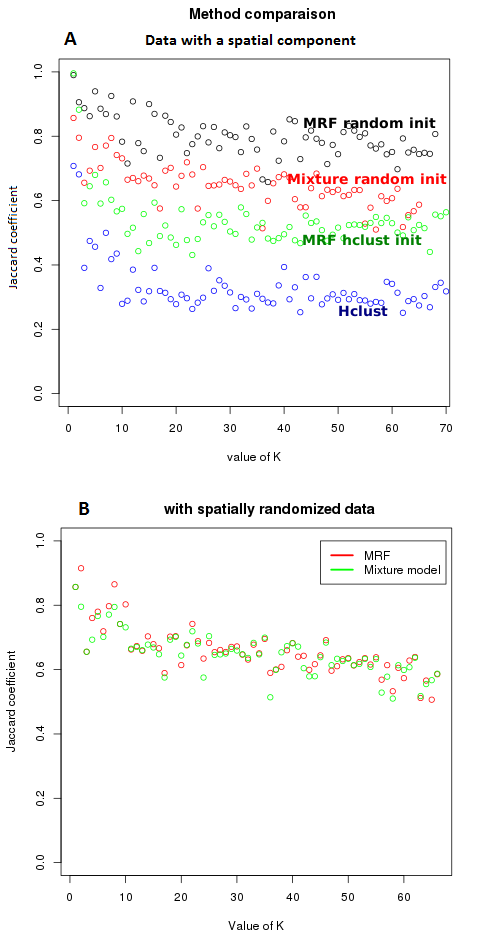
\includegraphics[width=0.9\linewidth]{gfx/chapter5/method_comparison.png}}
\caption{{\bf Jaccard coefficient between ``true" and resulting clusters on the simulated data with different methods and initializations.} Panel A compares the performance of the MRF method with a randomly initialization with an independent mixture model also with a random initialization, the MRF method initialized with the hClust classification and hClust alone on data simulated with a spatial component. Panel B shows the Jaccard coefficient for the MRF method and independent mixture model both with a random initialization; in this case both methods are applied to simulated data that lacks a spatial component.}
\label{fig:methodComparison}
	\end{figure}

Following this observation, for the rest of this thesis and especially in chapter \ref{ch:biology}, the HMRF method will be randomly initialized.

\section{Method performance compared to Hclust and independent mixture models}
 Because the simulated data provides a clear set of ``true" clusters and parameter values, it allows the HMRF clustering to be compared to other clustering methods in terms of clustering quality via the Jaccard coefficient. Additionally, computing time being a key factor for large datasets, I provide in this section some key figures about the execution time of the different methods.
	\subsection{Quality of the clustering results}
	
	The resulting Jaccard coefficients obtained by comparing the ``true" clusters and the clusters generated by different approaches are shown in Figure \ref{fig:methodComparison} for $\tilde{K} \in [4,70]$. The HMRF method, when used with a random initialization scheme, has an average Jaccard coefficient of $0.8$, and clearly demonstrates better performance than the other methods. The second best performing method is the independent mixture model with a random initialization, which has an average Jaccard coefficient of $0.7$. Since the independent mixture approach is equivalent to the MRF with all the $\beta$ parameters set equal to 0 (i.e., without a spatial component) this suggests that accounting for the spatial aspect yields improved results. hClust also performs relatively poorly with an average Jaccard coefficient around $0.4$.\\
	
	Although as mentioned previously, the Jaccard coefficient may not be linearly correlated with the quality of the clustering results because of the alignment step which can create biases, this simulation study seems to show that the HMRF consistently outperforms the other methods tested.
	
	
	\subsection{Computing time}
	As seen in the previous paragraph, I have assessed that the developed HMRF clustering method yields better results in terms of clustering than the other tested method. However, the fact that the method takes into consideration the spatial dependencies between data points, means that it is will be computationally more expensive than non spatial methods, especially as the number of sites increases.\\
	
	The number of clusters $K$ also has an important influence on the computing time. Given a fixed number of sites $S=32.203$, I ran the HMRF, and the mixture model methods on simulated datasets for $K \in [4,60]$ and have obtained on the same machine, the computing times shown in Figure \ref{fig:computing_time}.\\
	
	Because of the necessity to estimate the values of $\boldsymbol{\beta}$ at every step through a gradient ascent algorithm (see Chapter \ref{ch:HMRF}), and the increased complexity of computing the likelihood of the model when $K$ increases, it is unsurprising to see that the HMRF approach necessary computing time has an exponential relationship with $K$. On the other hand, the independent mixture model approach does not need to perform these calculations and exhibits a linear evolution. However, as seen in the previous paragraph, the spatial component of the model seems to improve significantly the clustering quality. Consequently, the HMRF approach might prove useful when $K$ is relatively low. Indeed, until $K=30$ the required computing time required for the HMRF is not dramatically higher compared to the mixture model approach. In practice, this is likely to be the case as complex biological tissues are not made of hundreds of sub-tissues. \\
	
	The computing time required for hClust is quite high as shown is Figure \ref{fig:computing_time} (blue line), but is constant for any number of clusters $K \in [2,S]$. Indeed, once the dendrogram is computed (see Chapter \ref{ch:non_spatial_clustering_visualization}), cutting the clustering tree to any number of clusters is trivial. It is also interesting to note that the clustering results for all values of $K$ are computed in one run with hClust when the other methods need a full run for each value of $K$. Although I have shown in Figure \ref{fig:methodComparison} that the clustering performances of hClust are clearly below those of the HMRF and the independent mixture models methods, the fact that the results for all values of $K$ are obtained at once, regardless of the relatively high computing time, might be advantageous in some cases. 
	
	\begin{figure}[h]
\centerline{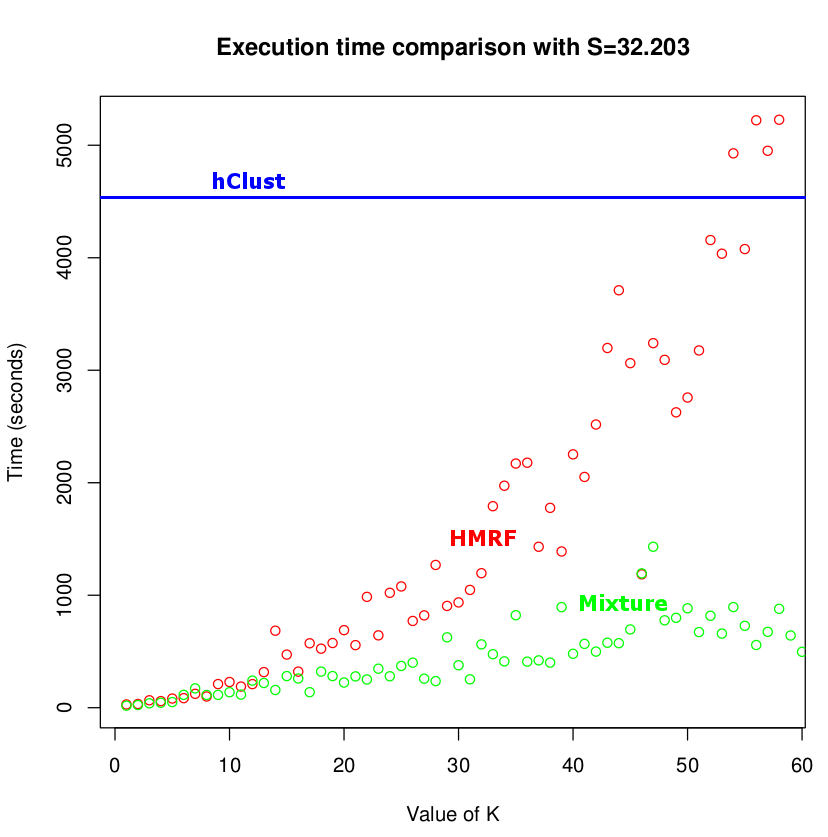
\includegraphics[width=0.8\linewidth]{gfx/chapter5/exec_time.png}}
\caption{{\bf Computing time required by different clustering methods for $K \in [4,60]$} On the x axis is shown the value of $K$ used to cluster the $32.203$ data points. The red dots represent the computing time required by the HMRF method, the green dots by an independent mixture model approach and the blue line for hClust.}
\label{fig:computing_time}
	\end{figure}
	
\section{summary}
In this chapter I have presented the simulation study conducted to evaluate the performances of the HMRF clustering method described in Chapter \ref{ch:HMRF}. Firstly, I have described the method used to simulate data with known spatial characteristics . Subsequently, I validated that all the parameters of the model were estimated correctly and consistently by the EM algorithm. I then discussed the performance of the method regarding the initialization scheme, and concluded that a selected random initialization yielded the best results. Finally I used the simulated data to compare the performances of the HMRF method compared to other clustering methods, the result of which was that even though the method is quite costly in terms of computing time when the number of clusters increases, it clearly outperforms both the independent mixture model and the hClust clustering methods in terms of accuracy.\\

The method validated, I will present in the next chapter the results obtained when the HMRF clustering was applied to the single cell in-situ hybridization data described in Chapter \ref{ch:singlecell}.


%*****************************************
%*****************************************
%*****************************************
%*****************************************
%*****************************************
